\documentclass{report}
\usepackage[utf8]{inputenc}
\usepackage{booktabs}
\usepackage{graphicx}
\usepackage[italian]{babel}
\usepackage{hyperref}
\usepackage[normalem]{ulem}
\usepackage{afterpage}
\useunder{\uline}{\ul}{}
\usepackage[margin=0.5in]{geometry} %serve per i margini dx e sx
\usepackage[utf8]{inputenc}
\usepackage{glossaries}
\usepackage[T1]{fontenc}
\usepackage{multirow}
\usepackage{float} 
\usepackage{tabularx}

\makeglossaries


\begin{document}
    \begin{figure}[htbp!]
    

    \centering\scshape\Medium\ UNIVERSITÀ DEGLI STUDI DI NAPOLI FEDERICO II \\
    \centering\scshape\small\ SCUOLA POLITECNICA E DELLE SCIENZE DI BASE\\
    \centering\scshape\Medium\ DIPARTIMENTO DI INGEGNERIA ELETTRICA E TECNOLOGIE DELL'INFORMAZIONE\\

        \begin{center}
            
\includegraphics[width=.30\textwidth]{Immagini/FedericoII.png}
        \end{center}
    \end{figure}
         \begin{center}

            
\includegraphics[width=.30\textwidth]{Immagini/Alexandria logo nome medium 2.png} 
        \end{center}
    \centering{\scshape\Large\bfseries\textbf{Progetto Bibliografia}}
        

    \begin{center}


        Giorgio Longobardo N86003571 \\ Claudio Simonelli N86003781\\ Giuseppe Francione N86003734\\~\\ Anno Accademico 2022/2023
    \end{center}
    
\hspace{0pt}
\vfill
    \raggedleft Docente:\\Di Martino\\Cutugno\\Starace
\vfill
\hspace{0pt}


    
    \newpage

    \tableofcontents

        \vspace*{\fill}
\centering{\textit{Questa pagina è stata lasciata intenzionalmente vuota.}}
    \chapter{Introduzione}
\raggedright{\section{Descrizione richiesta del progetto}}

È richiesto di migliorare e potenziare un sistema informativo già esistente per la gestione di bibliografie. Il sistema deve essere capace di salvare e organizzare i riferimenti bibliografici degli utenti.  In particolare, è possibile inserire, modificare, rimuovere riferimenti bibliografici di diverso tipo (e.g.: articoli scientifici su conferenza o rivista, libri, risorse on-line, dataset, etc.).
Ciascun riferimento è caratterizzato da un titolo univoco, un elenco di autori, una data, un URL (obbligatorio solo per risorse on-line), un DOI (facoltativo, ma univoco ove presente), e una descrizione testuale in cui l’utente può indicare aspetti significativi.
Inoltre, un riferimento può essere associato a un insieme di rimandi, ovvero di altri riferimenti presenti nel sistema che vengono menzionati nel testo.

Un utente, infine, può definire un insieme di categorie personalizzate e possibilmente gerarchiche, e associare ciascun riferimento a una o più categorie. Per organizzazione gerarchica delle categorie si intende la possibilità di specificare che una certa categoria (e.g.: “Informatica”) ha una o più sottocategorie (e.g.: “Basi di Dati” o “Testing”).

Non è possibile introdurre dipendenze cicliche, ovvero non è possibile che una categoria sia una sottocategoria (anche transitivamente) di sé stessa. L’appartenenza a una sottocategoria implica l’appartenenza a tutte le sue super-categorie. Non è pertanto possibile associare esplicitamente a un riferimento una categoria e una sua super-categoria.

Il sistema permette infine di effettuare interrogazioni avanzate, con possibilità di filtraggio per una o più categorie, per data, per parole chiave e per autore. Inoltre, è possibile ordinare i riferimenti per numero di citazioni ricevute, ovvero per il numero di volte in cui il riferimento è presente nei rimandi di altri riferimenti.

Inoltre è richiesto lo sviluppo di nuove funzionalità da integrare nel sistema informativo già esistente.

\raggedright{\section{Stato progetto originale}}
L'applicativo originale, seppur lasciato in ottimo stato, presenta alcuni punti deboli per quanto riguarda la progettazione software e usabilità. In particolare, verranno mostrati le varie funzionalità e i vari aspetti dell'applicativo che verranno modificati affinché possa rispettare gli standard odierni.
\raggedright{{\subsection{Basi di dati}}}
         \begin{center}
     \hspace{-1cm}
            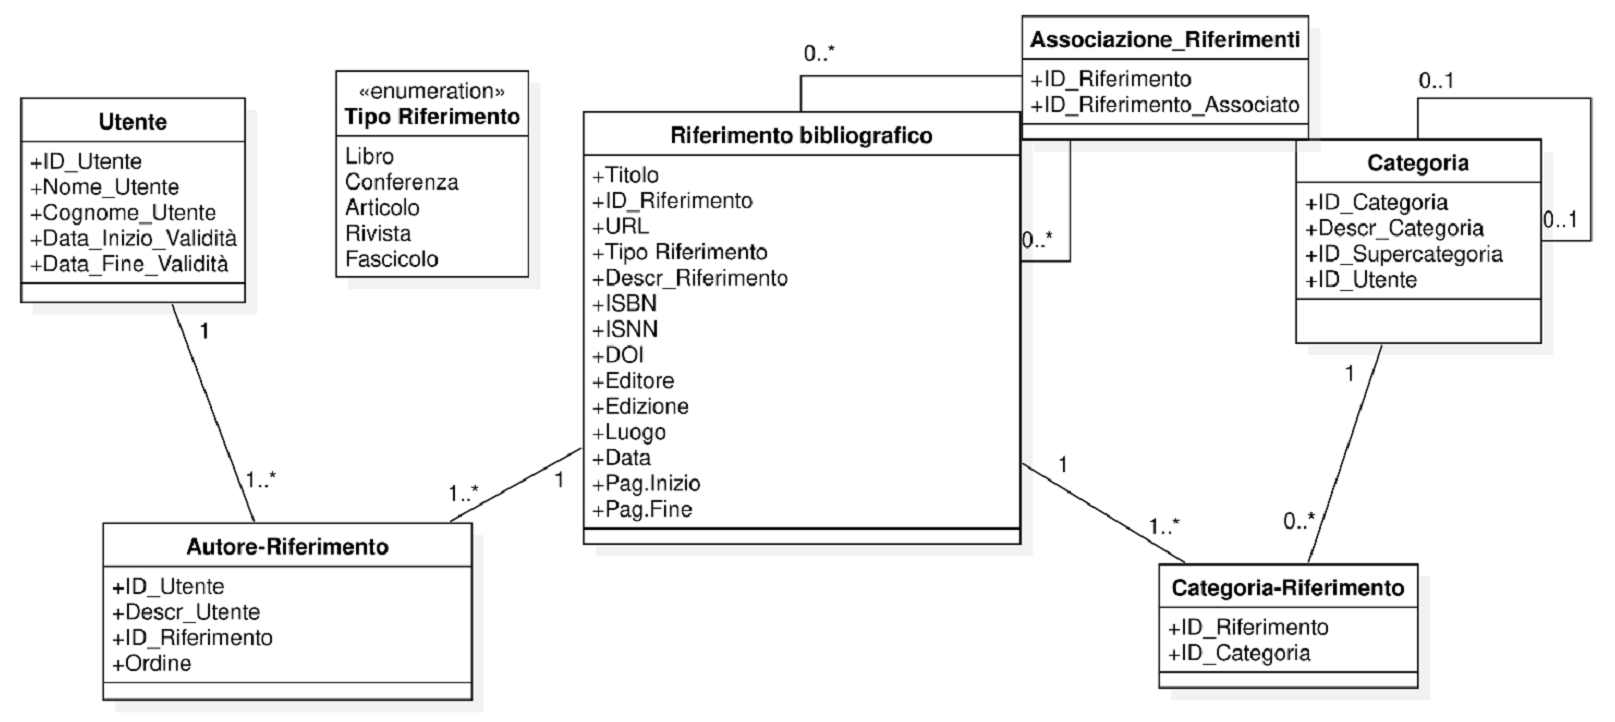
\includegraphics[width=.90\textwidth]{Immagini/VecchioProgetto/UML Basi di Dati pre ristrutturato.png} 
        \end{center}
La Basi di Dati originale è stata implementata nel modo seguente: \\la tabella \textit{Utente} descrive il possible utente che accede alla piattaforma dei riferimenti bibliografici. Contiene un identificativo univoco, un nome e cognome e due date di inzio e fine validità rispettivamente. \\
La tabella \textit{Autore-Riferimento} descrive il possible ideatore o relatore in base a che tipologia di riferimento bibliografico si analizzi. \\
La tabella \textit{Riferimento Bibliografico} descrive il possible riferimento bibliografico e le sue caratteristiche in base alla tipologia. \\
La tabella \textit{Categoria} descrive una categoria e le sue possibili sottocategorie. \\
La tabella \textit{Associazione-Riferimenti} è un descrittore di un riferimento che può essere associato a un insieme di rimandi. \\
La tabella \textit{Categoria-Riferimento} è un descrittore di una categoria che è associata ad  un riferimento. \\
\raggedright{\subsection{Applicativo Java}}
L’approccio di design utilizzato è quello di un sistema Object Oriented sviluppato in Java che dipende strettamente da un database PostgreSQL. L’ambiente di sistema è un qualsiasi sistema operativo non-mobile (quindi desktop) fornito di una connessione al database.
\begin{center}
    \hspace{-1cm}
        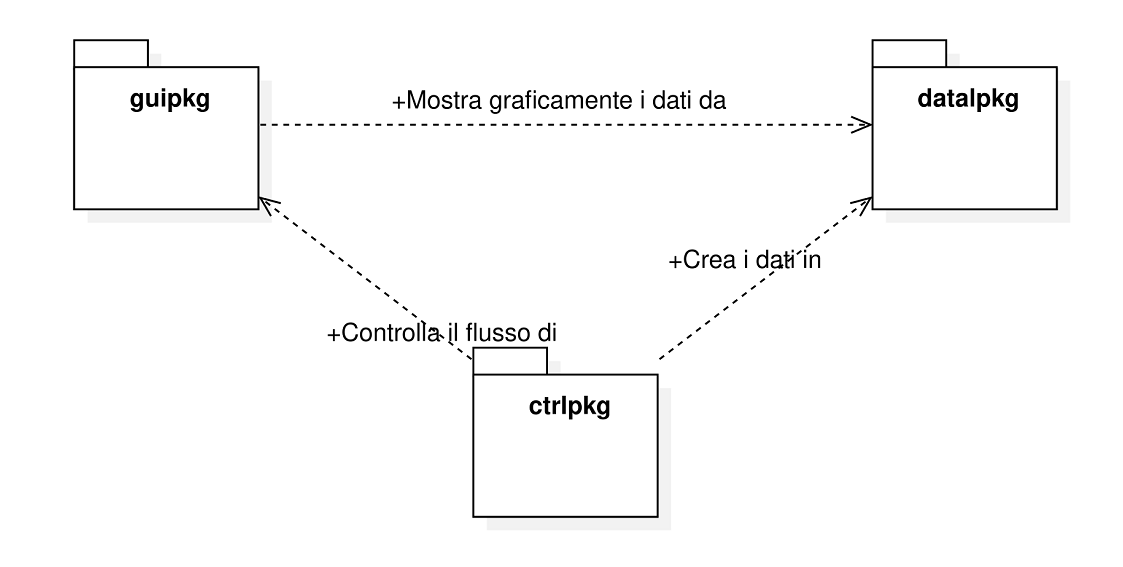
\includegraphics[width=.90\textwidth]{Immagini/VecchioProgetto/UML OO Java vecchioProgetto.png} 
\end{center}

Il sistema è costituito da 3 elementi principali, rappresentati in package: \\
\textit{guipkg}, per la definizione delle interfacce grafiche e le loro interazioni; \\ 
\textit{datalpkg}, per la definizione delle classi di dati che andranno trattati e mostrati;\\
\textit{ctrlpkg}, per la definizione dei collegamenti e delle varie interazioni tra sistema e database esterno.

\raggedright{\section{Migliorie del progetto originale e nuove funzionalità}}
La nuova versione del progetto prevede la modifica delle seguenti funzionalità:
\begin{itemize}
    \item Nuovo sistema di accesso: il sistema non prevederà l'utilizzo dell'ID utente ma di una email e password apposita. Durante la registrazione verrà richiesto infatti di inserire le due informaizoni che saranno poi salvate nel database. Inoltre, per preservare la sicurezza degli utenti, le password verranno criptate.
    \item Rimozione visibilità di ID accesso durante la registrazione: poiché l'utente non può più sapere il suo identificativo, non verrà mostrato il suo ID durante la registrazione.
    \item Potenziamento modalità di ricerca: la ricerca di riferimenti, citazioni e categorie verrà modificato e sarà più intuitivo ed efficiente.
    \item Apertura collegamenti: l'applicativo sarà capace di aprire gli URL inseriti per migliorare l'esperienza dell'utente, funzionalità mancante dell'applicativo originale.
    \item Impostazioni utente: verrà aggiunta la possibilità di modificare le proprie credenziali mediante un menù apposito.
    \item Miglioramento dell'interfaccia grafica: la GUI sarà totalmente ridisegnata per rispettare criteri di buona usabilità e con lo scopo di migliorare l'affordance iniziale, in tal modo da poter soddisfare più utenti possibili e di coprire tutte le possibili esigenze.
\end{itemize}

    
\newglossaryentry{Alexandria}
{
    name={Alexandria},
    description={Alexandria è un applicativo capace di gestire e creare i riferimenti bibliografici}
}

\newglossaryentry{riferimento}
{
    name={riferimento},
    description={Un riferimento è un collegamento ad un'opera bibliografica esistente dotato di nome, data, descrizione, codici univoci e di un eventuale URL per la visualizzazione}
}

\newglossaryentry{autore}
{
    name={autore},
    description={Un autore è una persona che ha prodotto un'opera da cui è poi tratto un riferimento presente nell'applicazione}
}

\newglossaryentry{categoria}
{
    name={categoria},
    description={Una categoria è un insieme contenente più riferimenti che trattano la stessa collezione di argomenti}
}

\newglossaryentry{sopra-categoria}
{
    name={sopra-categoria},
    description={Una sopra-categoria è un insieme contenente una o più categorie. La relazione che accomuna le categorie dell'insieme può essere varia e a scelta dell'utente. Infine, una sopra-categoria non può contenere se stessa o una categoria che ha già tale sopra-categoria come sopra-categoria}
}

\newglossaryentry{attributo}
{
    name={attributo},
    description={Un attributo è un dettaglio di un riferimento e può essere della seguente natura: uno o più codici univoci, il titolo del riferimento, la data di pubblicazione, una descrizione del riferimento, il nome dell'autore, il nome della casa editrice, il numero di edizione ed eventuale titolo a cui si riferisce}
}

\newglossaryentry{casi d'uso}
{
    name={casi d'uso},
    description={Un caso d'uso è una delle funzionalità principali del sistema. Senza di esse, l'applicativo non sarebbe completo e permette di svolgere una delle attività principali richieste}
}

\newglossaryentry{tipi di riferimento}
{
    name={tipo di rifeirmento},
    description={Un tipo di riferimento è il tipo di formato del riferimento pubblicato e può assumere diversi tipi, ovvero: un libro, un articolo, un fascicolo, una rivista, una conferenza. La conferenza può essere di formato visivo virtuale}
}

\newglossaryentry{tipo di ricerca}
{
    name={tipo di ricerca},
    description={Il tipo di ricerca determina in \textit{quale modo} debba essere ricercato un determinato riferimento e può essere per titolo (mostra solo i riferiementi avente tale titolo), per autore (mostra tutti i riferimenti di quel determinato autore) e per DOI (mostra i riferimenti avente quel determinato DOI)}
}

\newglossaryentry{DOI}
{
    name={DOI},
    description={Un DOI è un codice univoco digitale di un particolare riferimento.}
}

\newglossaryentry{layer}
{
    name={Layer},
    description={Un layer è uno strato dell'architettura del sistema. Può essere gerarchico e svolge una determinata attività o compito.}
}

\newglossaryentry{HTTP}
{
    name={HTTP},
    description={HTTP è un protocollo per la comunicazione delle informazioni fra client-server. In Alexandria, essa è utilizzata per la comunicazione fra l'applicativo e il DBMS}
}

\newglossaryentry{REST}
{
    name={REST},
    description={Representational state transfer è uno stile architetturale per sistemi distribuiti. In questo caso, è la rappresentazione dell'Architettura di Alexandria.}
}

\newglossaryentry{DBMS}
{
    name={DBMS},
    description={Un DBMS (Database management system) è un sistema di gestione di una base di dati, in particolare per la creazione, manipolazione e ricerca dei dati. In Alexandria, si riferisce a PostgreSQL, un DBMS di tipo relazionale.}
}


\newglossaryentry{front end}
{
    name={Front-End},
    description={Il front end è l'insieme di tutte le attività e operazioni che l'utente finale deve compiere o vedere.}
}

\newglossaryentry{API}
{
    name={API},
    description={Un'API è un'interfaccia di programmazione di un'applicazione, ovvero un insieme di librerie e framework atte a implementare determinate funzionalità o un sottosistema. In Alexandria, abbiamo implementato un'API apposita per la ricerca efficiente dei riferimenti.}
}

\newglossaryentry{Spring Boot}
{
    name={Spring Boot},
    description={Spring Boot è un'API rest per l'implementazione, appunto, di un applicativo basato su REST.}
}

\newglossaryentry{Weak Equivalence Class Testing}
{
    name={Weak Equivalence Class Testing},
    description={La WECT è un processo di copertura che stabilisce che p er ogni classe di equivalenza
ci deve essere un Test case che usa un valore nominale da quella classe
di equivalenza.}
}

\printglossaries


    \chapter{Requisiti Software}
\raggedright{\section{Modellazione casi d'uso richiesti}}
\raggedright{\subsection{Autenticazione}}
\raggedright{\subsection{Ricerca Riferimenti}}
\raggedright{\subsection{Ricerca Autori}}
\raggedright{\subsection{Crea Riferimenti}}
\raggedright{\subsection{Crea Categorie}}
\raggedright{\subsection{Visualizza e modifica categorie}}






\raggedright{\section{Individuazione target degli utenti}}

\raggedright{\section{4 casi d'uso in particolare}}

\raggedright{\section{MockUp Interfaccia grafica}}

\raggedright{\section{Valutazione dell'usabilità}}

\raggedright{\section{Glossario}}

\raggedright{\section{Classi, oggetti e relazioni d'analisi}}

\raggedright{\section{Diagrammi di Sequenza}}

\raggedright{\section{Prototipazione funzionale}}










    \chapter{Design del Sistema}
\raggedright{\section{Analisi dell'architettura e motivazioni}}
L'architettura del software precedente era strutturata in maniera tale che fosse monolitica: era composta da tre strati gerarchici, dove il più basso, la View, era il \gls{layer} deputato al \gls{front end}, il layer centrale, i Model, era deputato alla gestione dei modelli richiesti dal sistema e infine il layer Database, che gestiva la manipolazione dei dati ed eventuale loro creazione, rimozione o modifica. \\
In Alexandria, nella fase di progettazione dell'architettura del sistema, il compito più arduo è stato quello di mantenere il Database e riutilizzare il codice sorgente ma ristrutturare l'architettura per renderla più flessibile e non monolitica, in particolare di adottare l'architettura \gls{REST}. Il sistema infatti prevede più sottoinsiemi di layer che collettivamente compongono l'applicativo: il front end è composto da tre layer, uno per la comunicazione \gls{HTTP} con il server, uno per l'interfaccia grafica e un'altra per la modellazione delle classi richieste. Il layer per la comunicazione a sua volta è composto da un layer aggiuntivo per la corretta gestione dei dati, utilizzato solamente dal front end nella trasmissione dei dati o per la richiesta di lettura. L'intero sottosistema del front end è inglobato nell'architettura \gls{REST} che comprende anche il lato server. Quest'ultimo infatti rispecchia la rappresentazione di una architettura REST basata su HTTP, dove lo stato dell'applicazione e le funzionalità sono divisi in risorse, ogni risorsa è unica e indirizzabile usando sintassi universale per uso nei link ipertestuali. Tutte le risorse sono condivise come interfaccia uniforme per il trasferimento di stato tra front end e risorse, questo consiste in un insieme vincolato di operazioni ben definite, un insieme vincolato di contenuti, opzionalmente supportato da codice a richiesta.
Abbiamo deciso di implementare un'architettura REST per la versatilità di richiedere e trasmettere le risorse al server, per la falicità del mapping del Database nelle entità e soprattuto perché perfetto per le nostre esigenze: il database durante la fase di progettazione già era implementato, ma non era completamente utilizzabile per via dell'architettura monolitica del precedente sistema. L'API Rest si è presentata come un'ottima scelta per poter implementare un nuovo sistema senza dover realizzare dal nulla lo stesso database.

\raggedright{\section{Descrizione e motivazioni delle scelte tecnologiche adottate}
Le tecnologie usate durante lo sviluppo del progetto sono essenzialmente tre: PostgreSQL per il Database Management System, Spring Boot per l'API Rest da implementare per la comunicazione con il DBMS e Flutter per lo sviluppo del front-end. Di seguito descrizione e motivazioni delle nostre scelte.

\raggedright{\subsection{PostgreSQL}}
PostgreSQL è un \gls{DBMS} di tipo relazionale in cui è possibile inserire dati, modificarli,  ricercarli ed eliminarli. E' inoltre fornito di funzionalità aggiuntive come la creazione di funzioni tramite PLPGSQL o SQL Dinamico. \\
In Alexandria, il back-end è gestito in parte da PostgreSQL. Il motivo principale di questa scelta è la già nota esistenza di un Database apposito e le modifche pensate durante la fase di progettazione non erano tali da dover reimplementare interamente il Database. Non avrebbe avuto senso dover reimplementare lo stesso database con le stesse funzioni per un nuovo DBMS, perdendo così tempo per la progettazione dell'applicativo, anche perché il Database risultava perfettamente funzionante durante la fase di testing del vecchio applicativo. \\
Il DBMS ci ha permesso di implementare funzioni apposite per determinate query, soprattutto per le relazioni ricorsive, tipi enumerativi e cast dedicati, funzionalità che magari non erano presenti in altri DBMS. \newpage
\raggedright{\subsection{Spring Boot JPA}}
\gls{Spring Boot} è un API Rest atto a implementare un applicativo capace di comunicare mediante archiettura REST. \\
In Alexandria, Spring Boot è stato uno strumento fondamentale per l'implementazione e la gestione delle risorse dal client al DBMS. Prima dell'implementazioen effettiva, abbiamo avuto dinanzi una vaste alternative di framework per l'implementazione di tale architettura. La scelta finale è però ricaduta su Spring Boot principalmente per due motivi: dato che l'applicativo originale era stato scritto in Java, ci è risultato più conveniente implementare Spring Boot su un eseguibile Java essendo possibile poter recuperare il codice sorgente originale e modificarlo all'occorrenza. Inoltre, Spring Boot offre la possibilità di effettuare query native, oltre a quelle di supporto: in tal modo abbiamo potuto riportare uno a uno le query già implementate nel vecchio sistema, senza doverle reimplementare. L'unico sforzo effettivo è stato quello di adattare le funzioni di query per ogni caso.  \\
\raggedright{\subsection{Flutter}}
Flutter è un framework open source per la creazione delle interfacce native per diversi sistemi operativi, tra cui Android. \\
Una delle motivazioni principali della scelta dell'utilizzo di Flutter è la sua enorme semplicità nella creazione e modifica delle interfacce grafiche. Inoltre, è fornito nativamente il supporto per la maggior parte dei sistemi operativi in uso, così, se si dovesse esportare Alexandria su nuove piattaforme, basterà solamente compilare il codice sorgente e distribuire l'applicativo. In caso di modifiche alle schermate in base alle esigenze del dispositivo che lo richiede, basterà modificare i metodi appositi, senza dover ricorrere ad artifizi particolari. Infine, essendo un linguaggio particolarmente simile a Java, è stato semplice dover esportare il codice originale in Flutter, modificando però opportunamente il codice in caso di incompatibilità.

\raggedright{\section{Diagrammi delle classi di design}}

        \begin{center}
            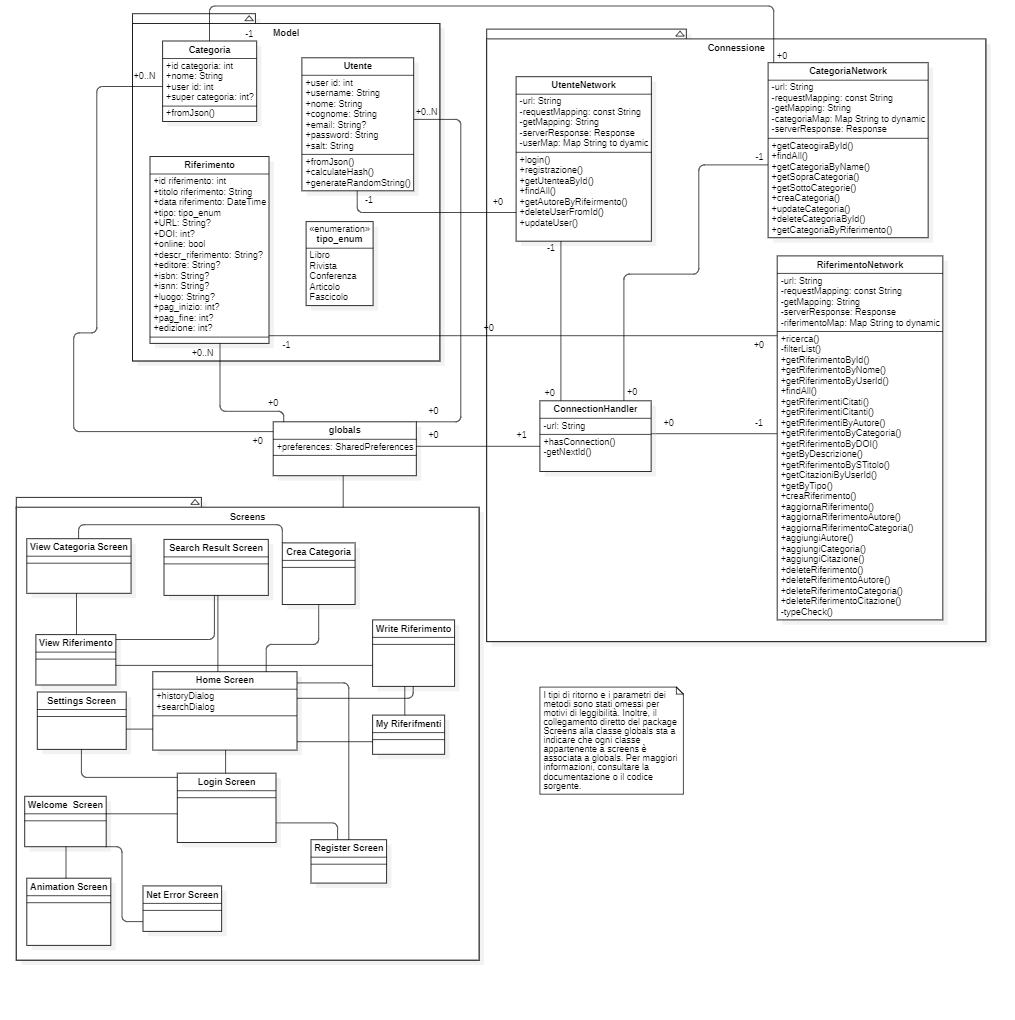
\includegraphics[width=1.0\textwidth]{Immagini/Alexandria/UML Design.PNG} 
        \end{center}

\raggedright{\section{Diagrammi di sequenza di design}}

\raggedright{\section{Codice sorgente e Dockerfile}}

    \chapter{Testing e valutazione sul campo dell'usabilità}
\raggedright{\section{Codice xUnit}}
Di seguito viene riportato il codice dartUnit per 4 metodi non banali che abbiano almeno due parametri.\\

\raggedright{\subsection{Unit Testing: Creazione Categoria}}
\lstinputlisting[language=Java]{dartUnit/creaCategoria.dart}

\newpage
\raggedright{\subsection{Unit Testing: Ricerca di un Riferimento}}
\lstinputlisting[language=Java]{dartUnit/ricercaRiferimento.dart}
\newpage
\raggedright{\subsection{Unit Testing: Calcolo hash}}
\lstinputlisting[language=Java]{dartUnit/calcoloHash.dart}
\raggedright{\subsection{Unit Testing: Regitrazione}}
\lstinputlisting[language=Java]{dartUnit/registrazione.dart}
\newpage
\raggedright{\subsection{Strategie adottate per la progettazione dei test}}
Tali unità di test sono state implementate mediante un approccio Black Box, anche se il codice sorgente era ovviamente disponibile. Questo perché abbiamo preferito testare il comportamento esterno dell'applicativo, senza doverci focalizzare sulle sfaccettature del codice. \\
Abbiamo deciso di presentare quattro unità di test tra i tanti metodi che sarebbero stati maggiormente utilizzati in Alexandria: un metodo per la creazione di una categoria, uno per la ricerca di un riferimento, uno per la creazione di un riferimento e infine uno per l'aggiunta di una citazione. In particolare, sono stati individuate tali classi d'equivalenza:

\begin{table}[H]
\begin{tabular}{|l|l|l|l|}
\hline
\textbf{creazioneCategoria}  &                           &                           &                          \\ \hline
String nome         & CE1: \{""\} n. v.         & CE2: \{"abc"\} val.       &                          \\ \hline
int user\_id        & CE3: \{minInt, -1\} n. v. & CE4: \{0, maxInt\} val.   &                          \\ \hline
int? superCategoria & CE5: \{null\} val.        & CE6: \{minInt, -1\} n. v. & CE7:  \{0, maxInt\} val. \\ \hline
\end{tabular}
\end{table}

\begin{table}[H]
\begin{tabular}{|l|l|l|l|}
\hline
\textbf{ricercaRiferimento}                      &                       &                              &                                \\ \hline
String? titolo                          & CE1: \{null\} val.    & CE2: \{""\} n. v.            & CE3: \{"abc"\} val.            \\ \hline
int? doi                                & CE4: \{null\} val.    & CE5: \{minInt, maxInt\} val. &                                \\ \hline
List\textless{}Categoria\textgreater c  & CE6: \{{[}{]}\} val.  & CE7: \{{[}1, .., n{]}\} val. &                                \\ \hline
List\textless{}tipo\_enum\textgreater t & CE8: \{{[}{]}\} n. v. & CE9: \{{[}1, .., 5{]}\} val. & CE10: \{{[}6, .., n{]}\} n. v. \\ \hline
\end{tabular}
\end{table}

\begin{table}[H]
\begin{tabular}{|l|l|l|}
\hline
\textbf{registrazioneUtente}     &                           &                         \\ \hline
String username         & CE1: \{""\} n. v.       & CE2: \{"abc"\} val.     \\ \hline
String unhashedPassword & CE3: \{""\} n. v. & CE4: \{"abc"\} val. \\ \hline
String nome             & CE5: \{""\} n. v.         & CE6: \{"abc"\} val.     \\ \hline
String cognome          & CE7: \{""\} n. v.         & CE8: \{"abc"\} val.     \\ \hline
String email            & CE9: \{""\} n. v.         & CE10: \{"abc"\} val.    \\ \hline
\end{tabular}
\end{table}
\begin{table}[H]
\begin{tabular}{|l|l|l|}
\hline
\textbf{calculateHash}  &                           &                         \\ \hline
String unhashedPassword & CE1: \{""\} n. v.       &  CE2: \{"abc"\} val.                       \\ \hline
String salt    & CE3: \{""\} n. v. & CE4: \{"abc"\} val. \\ \hline
\end{tabular}
\end{table}
Il criterio di copertura utilizzato è la \textit{\gls{Weak Equivalence Class Testing}}.
Le caratteristiche individuate per ogni classe d'equivalenza rispecchiano i casi limite dei possibili valori che un parametro della funzione possa assumere. 
\newpage
\raggedright{\section{Valutazione dell'usabilità sul campo}}
A prodotto finito, ci siamo avvalsi dell'uso di \href{https://analytics.google.com/analytics/web/}{Google Analytics} per analizzare in dettaglio le interazioni con gli utenti e il comportamento dell'applicazione una volta collegato con il server \gls{AWS}. In particolare, sono stati generati i seguenti file di log durante le fasi di valutazione dell'usabilità:

\begin{figure}[H]
    \centering
    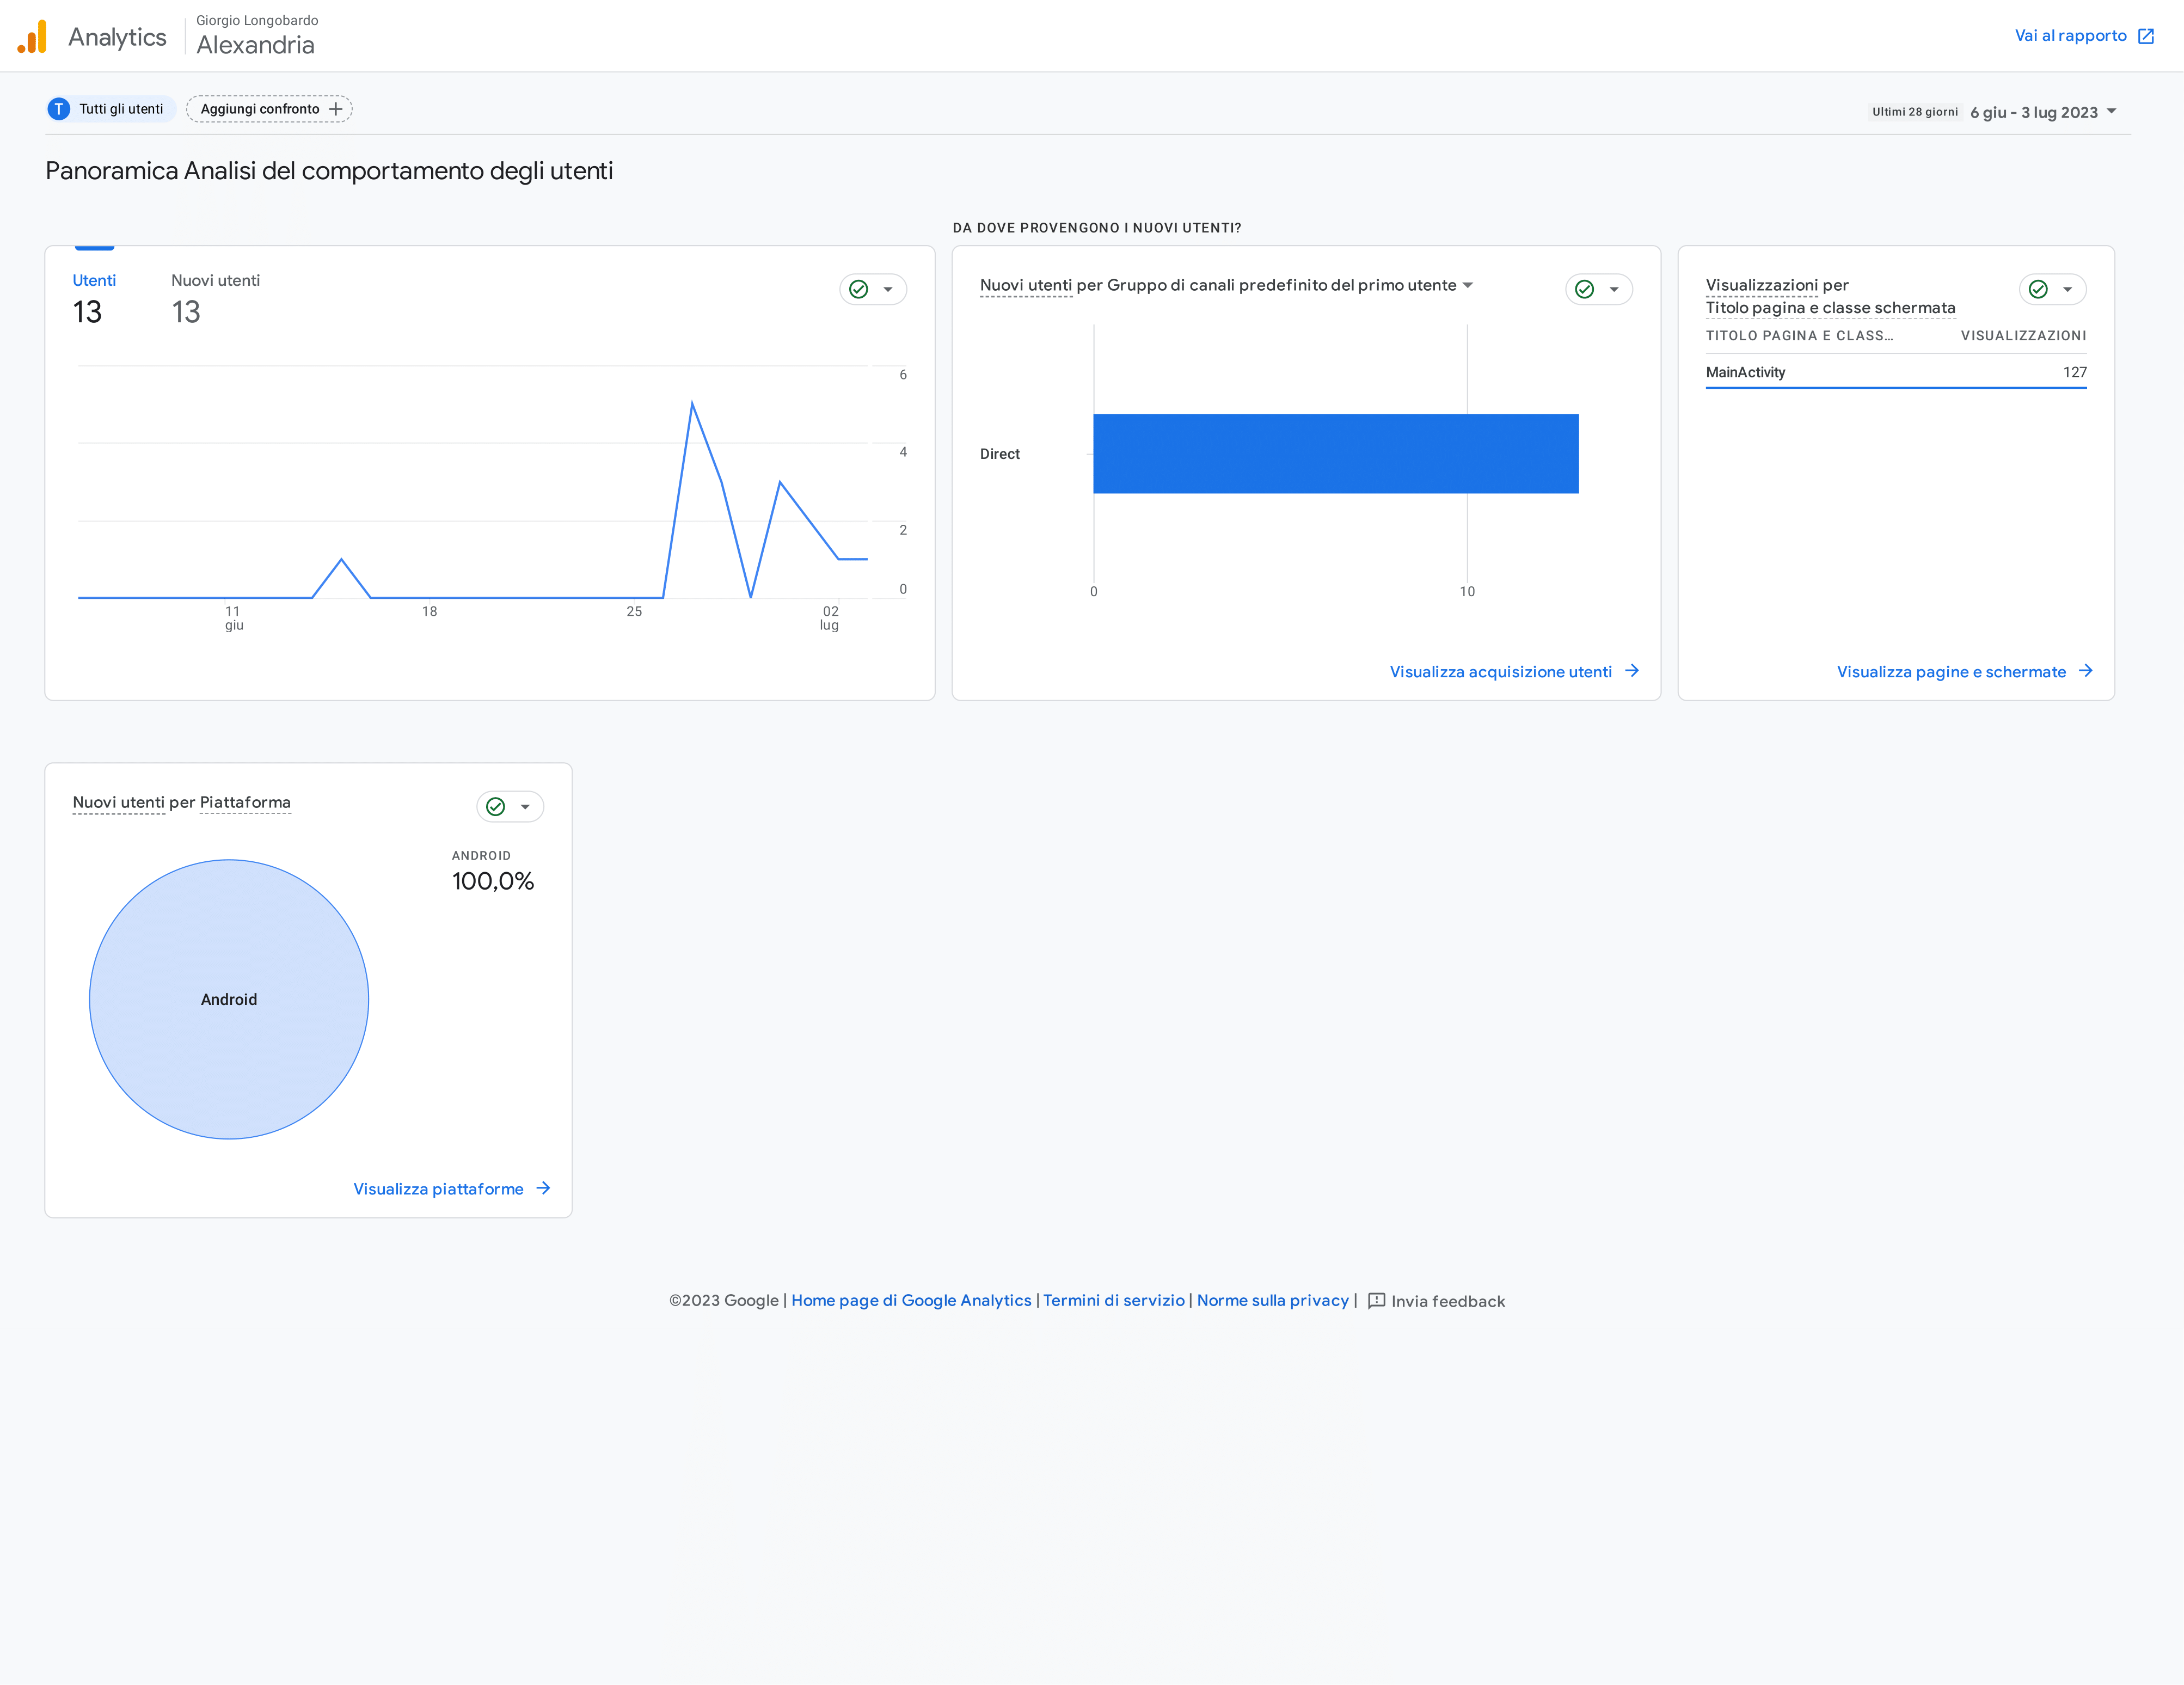
\includegraphics[width=0.99\textwidth]{Immagini/Alexandria/Report/panoramica-1.png}
    \caption{Panoramica generale}
\end{figure}

\begin{figure}[H]
    \centering
    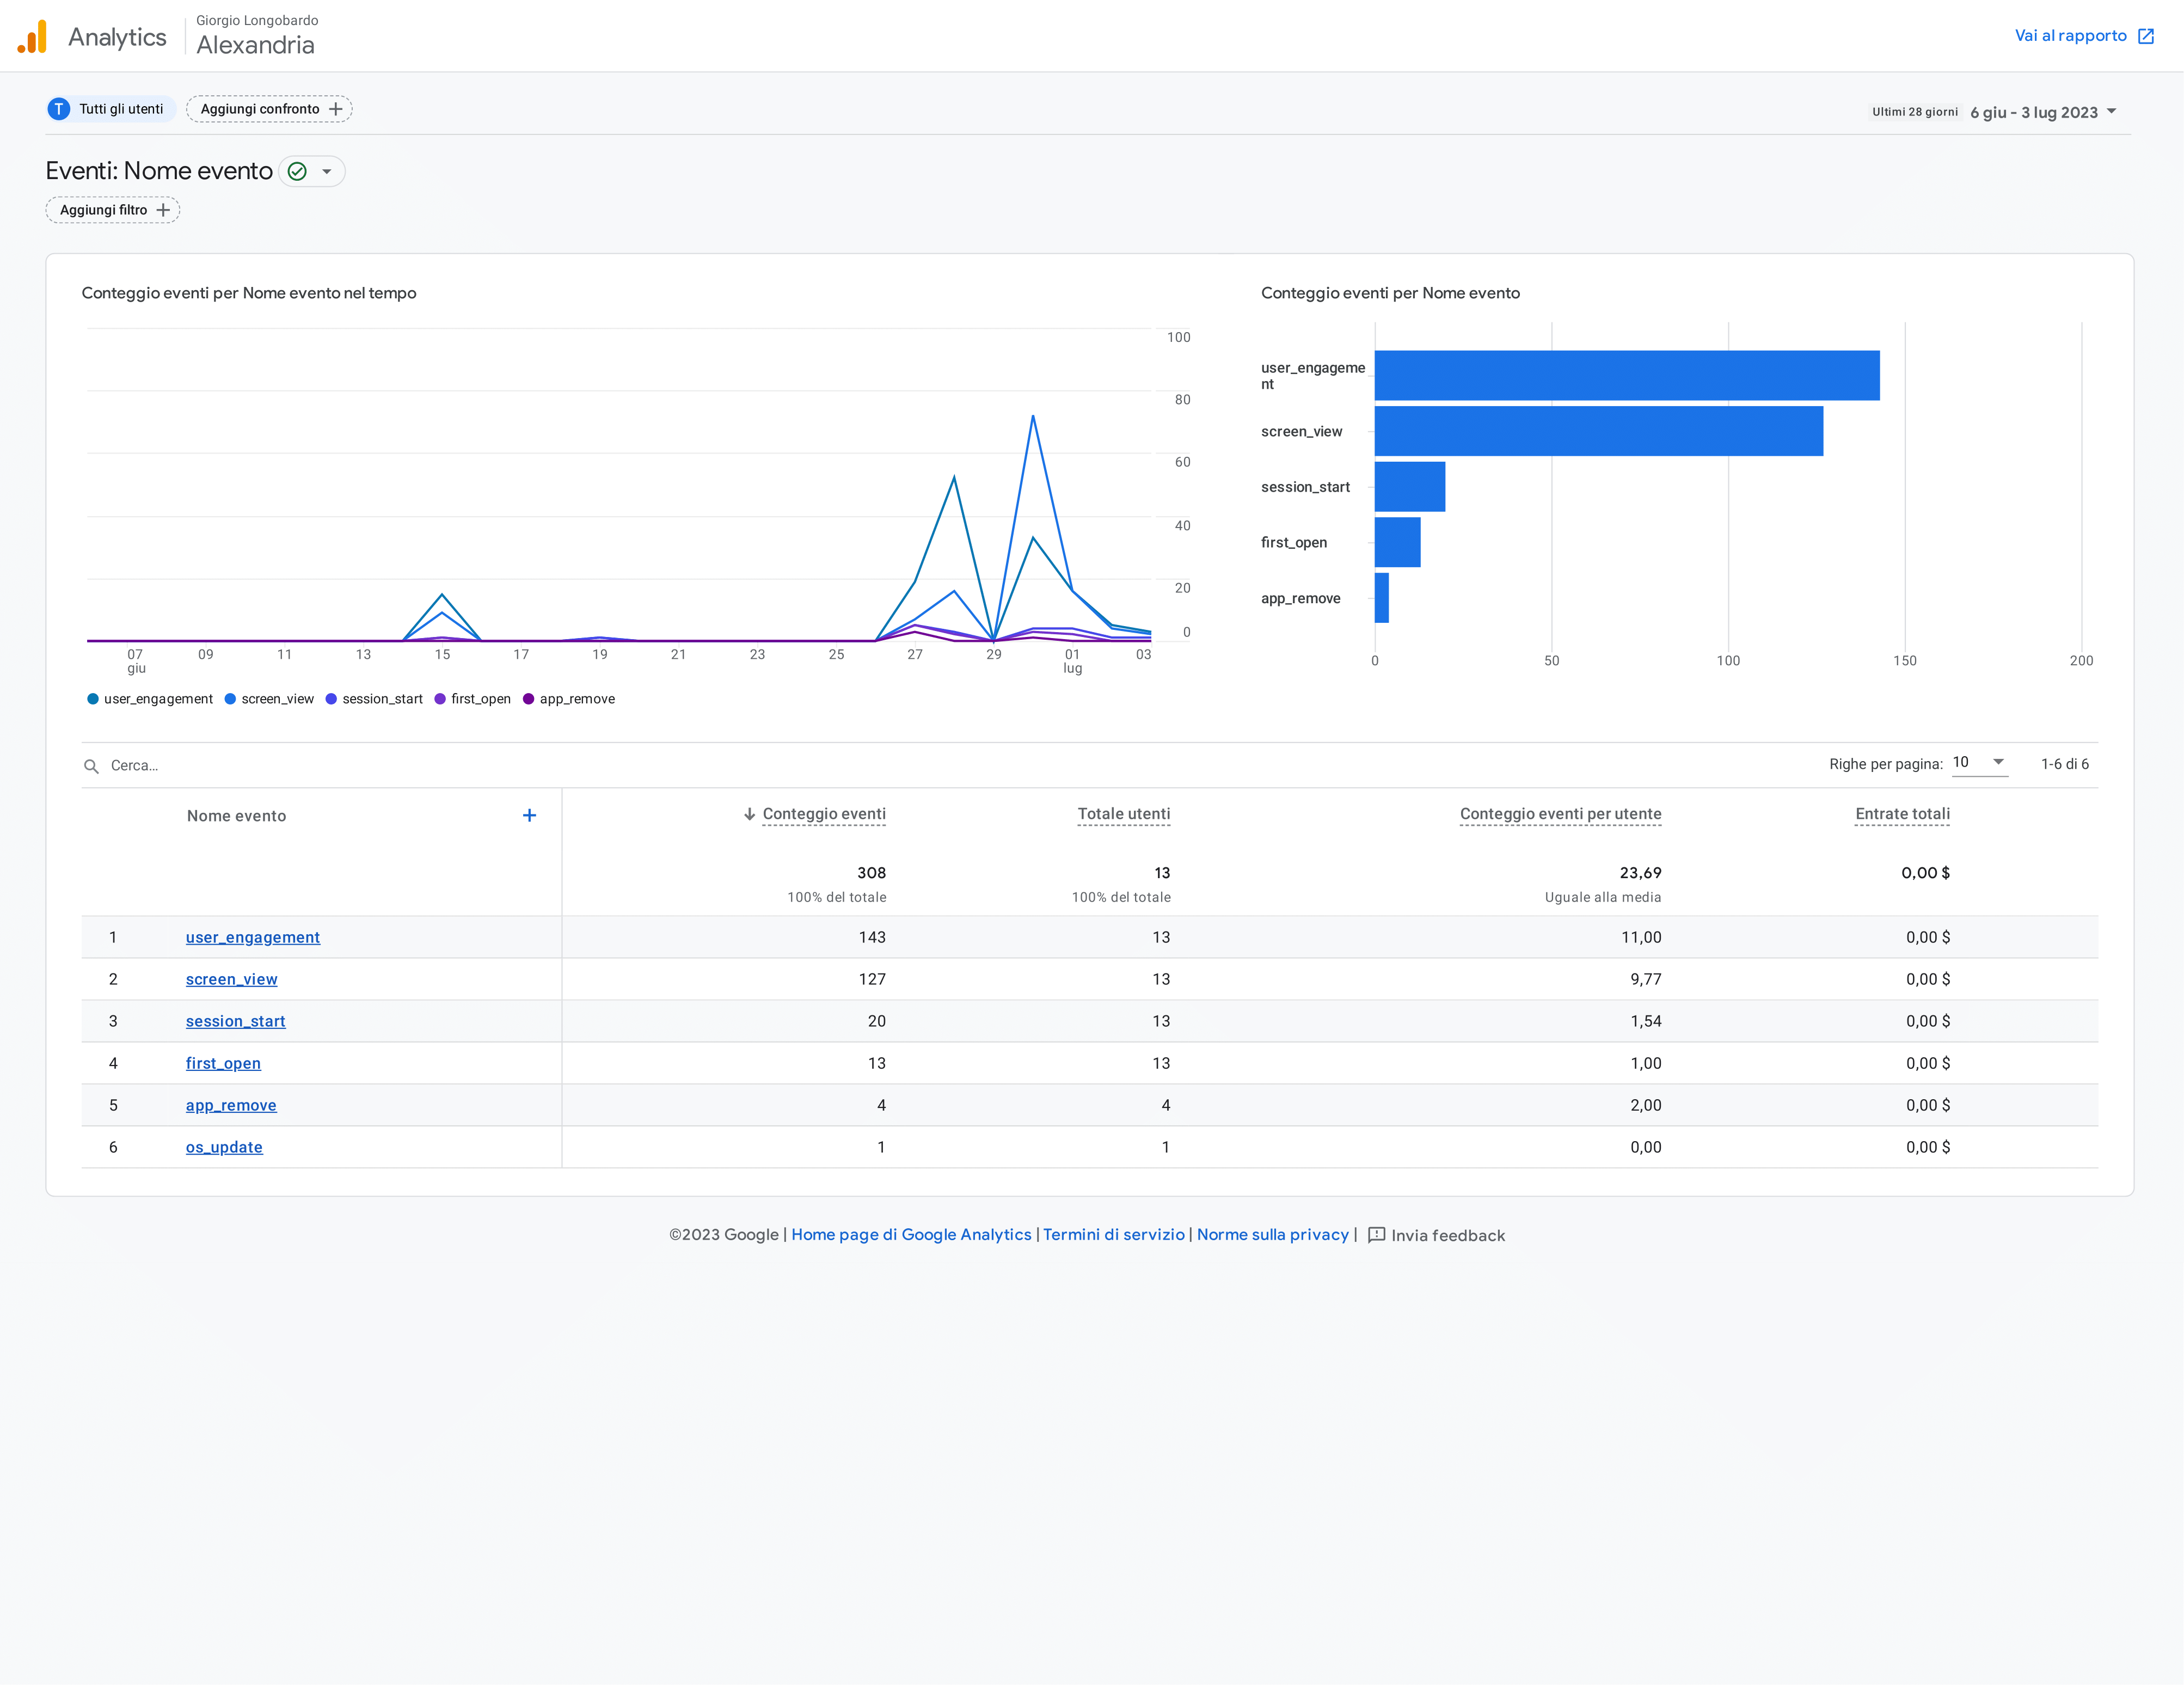
\includegraphics[width=0.99\textwidth]{Immagini/Alexandria/Report/eventi-1.png}
    \caption{Panoramica degli eventi}
\end{figure}

\begin{figure}[H]
    \centering
    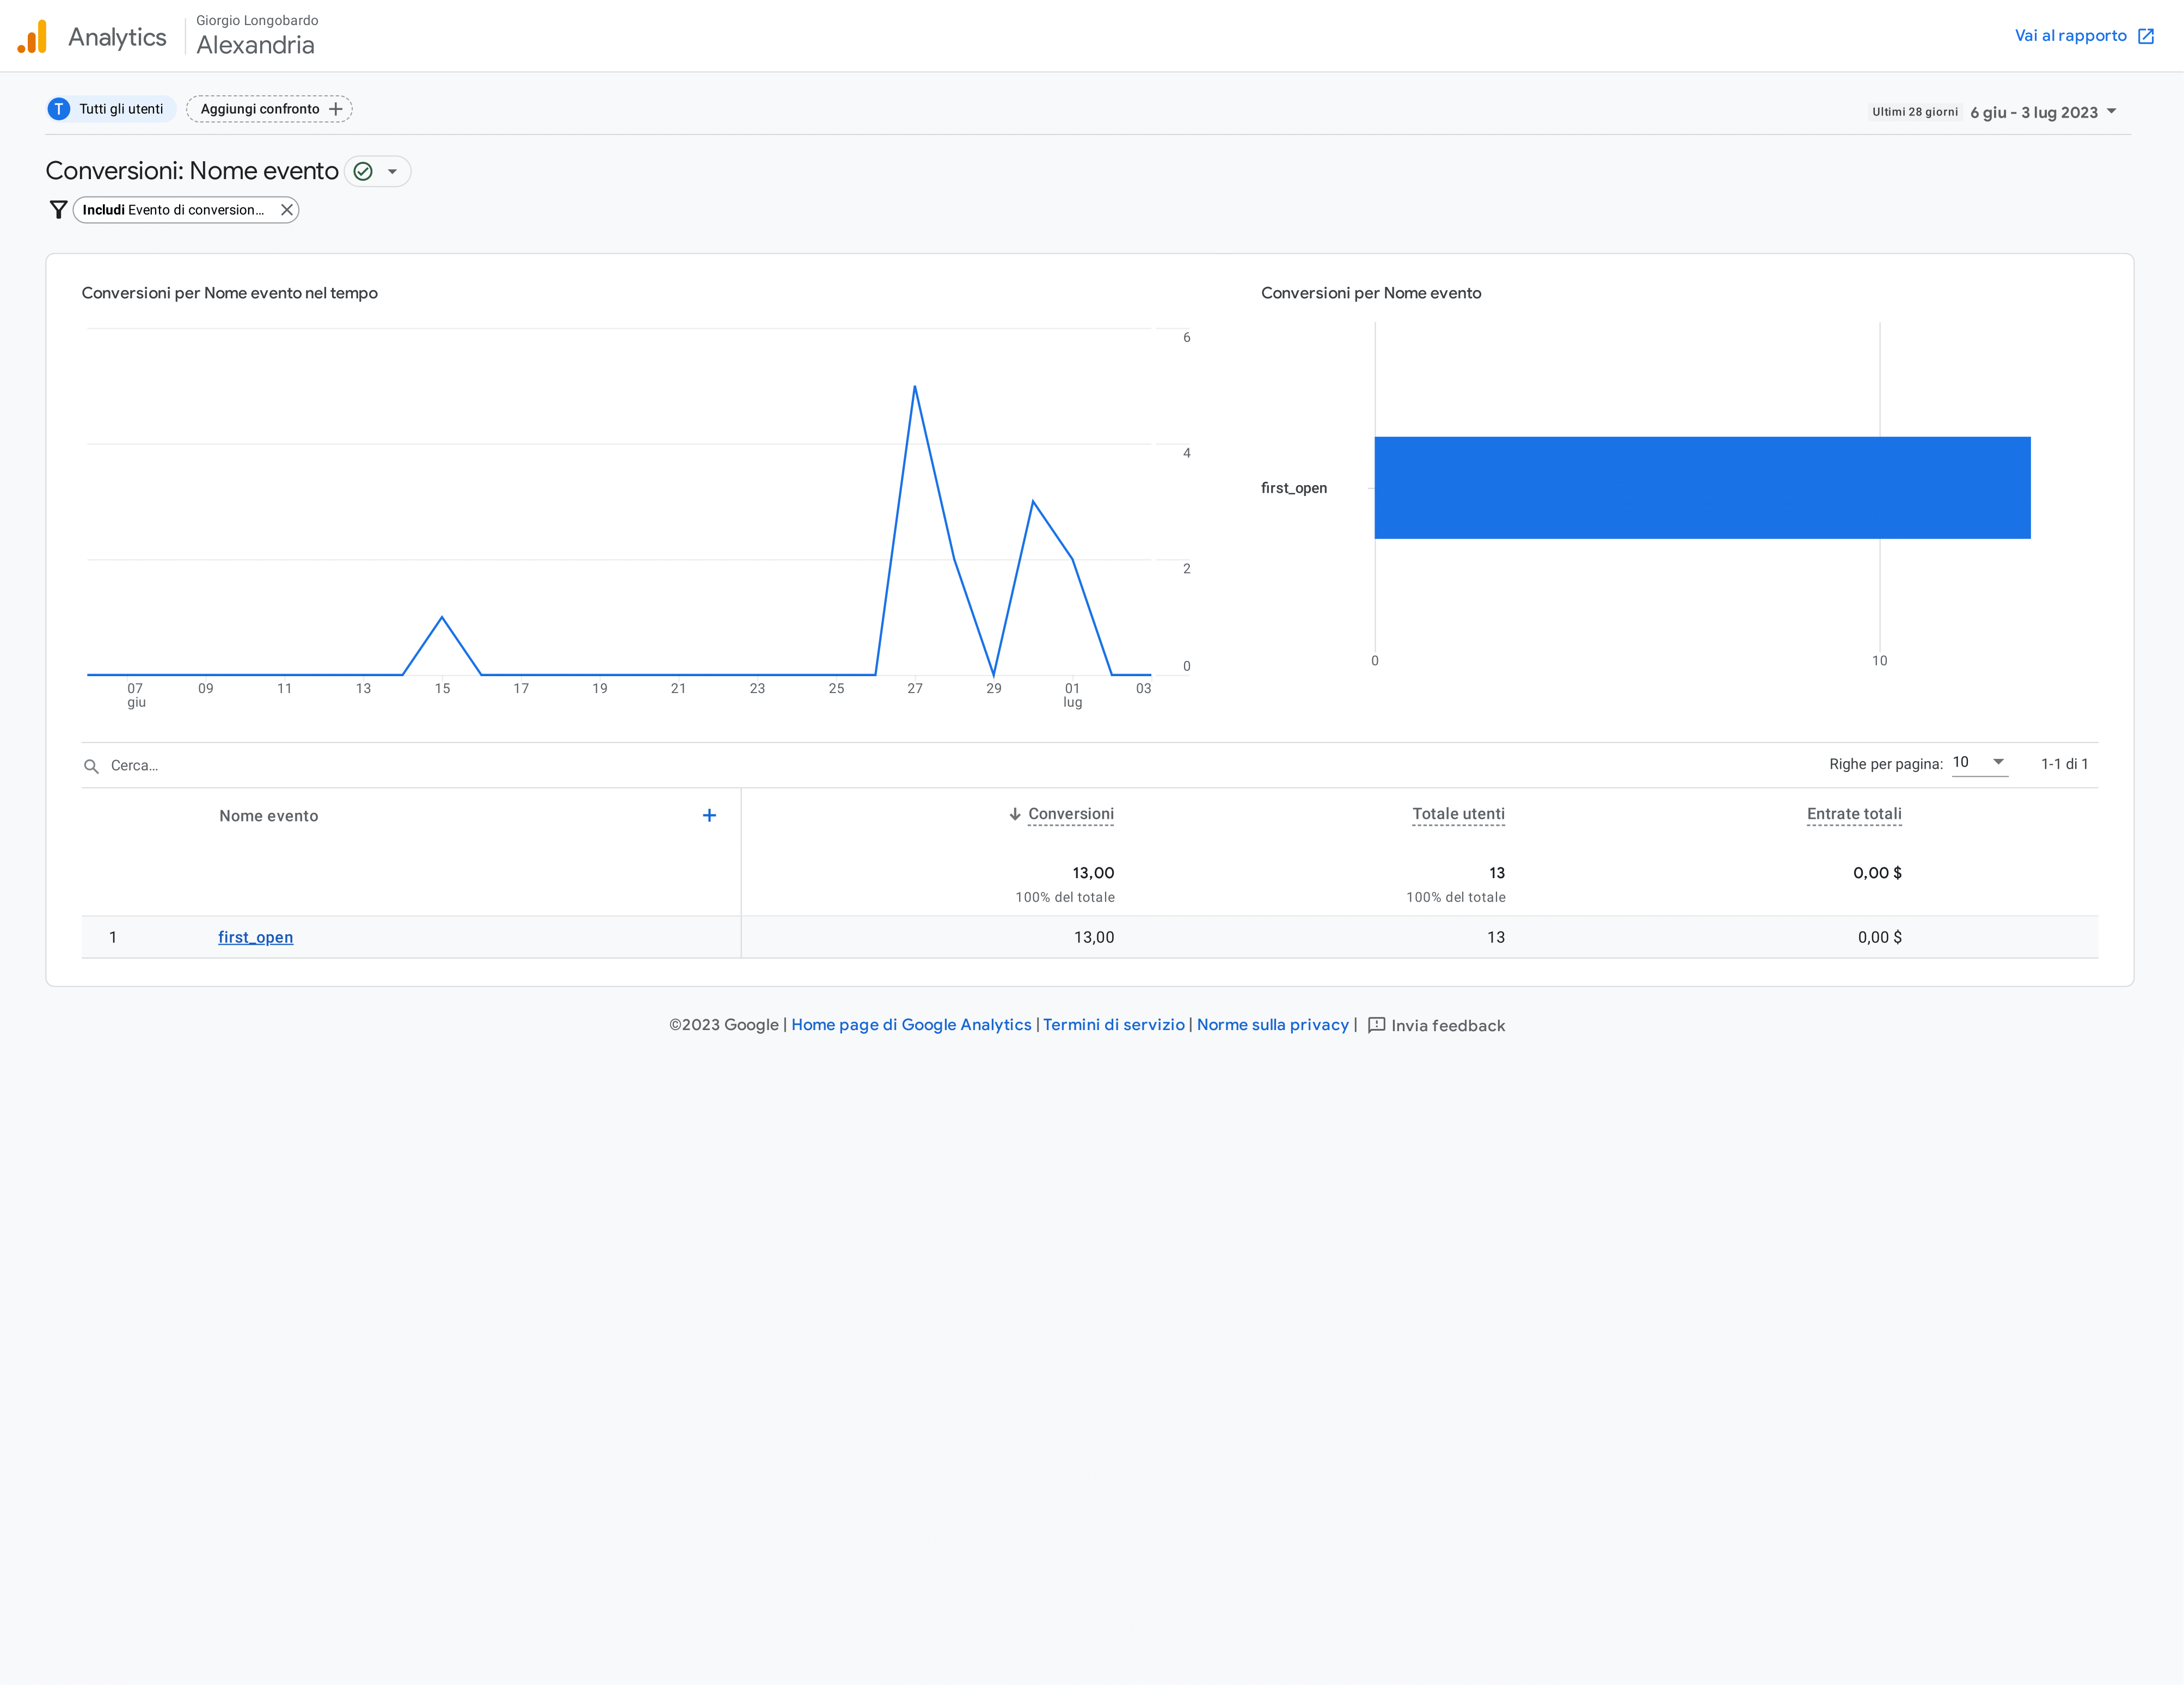
\includegraphics[width=0.99\textwidth]{Immagini/Alexandria/Report/conversioni-1.png}
    \caption{Panoramica delle conversioni}
\end{figure}

\begin{figure}[H]
    \centering
    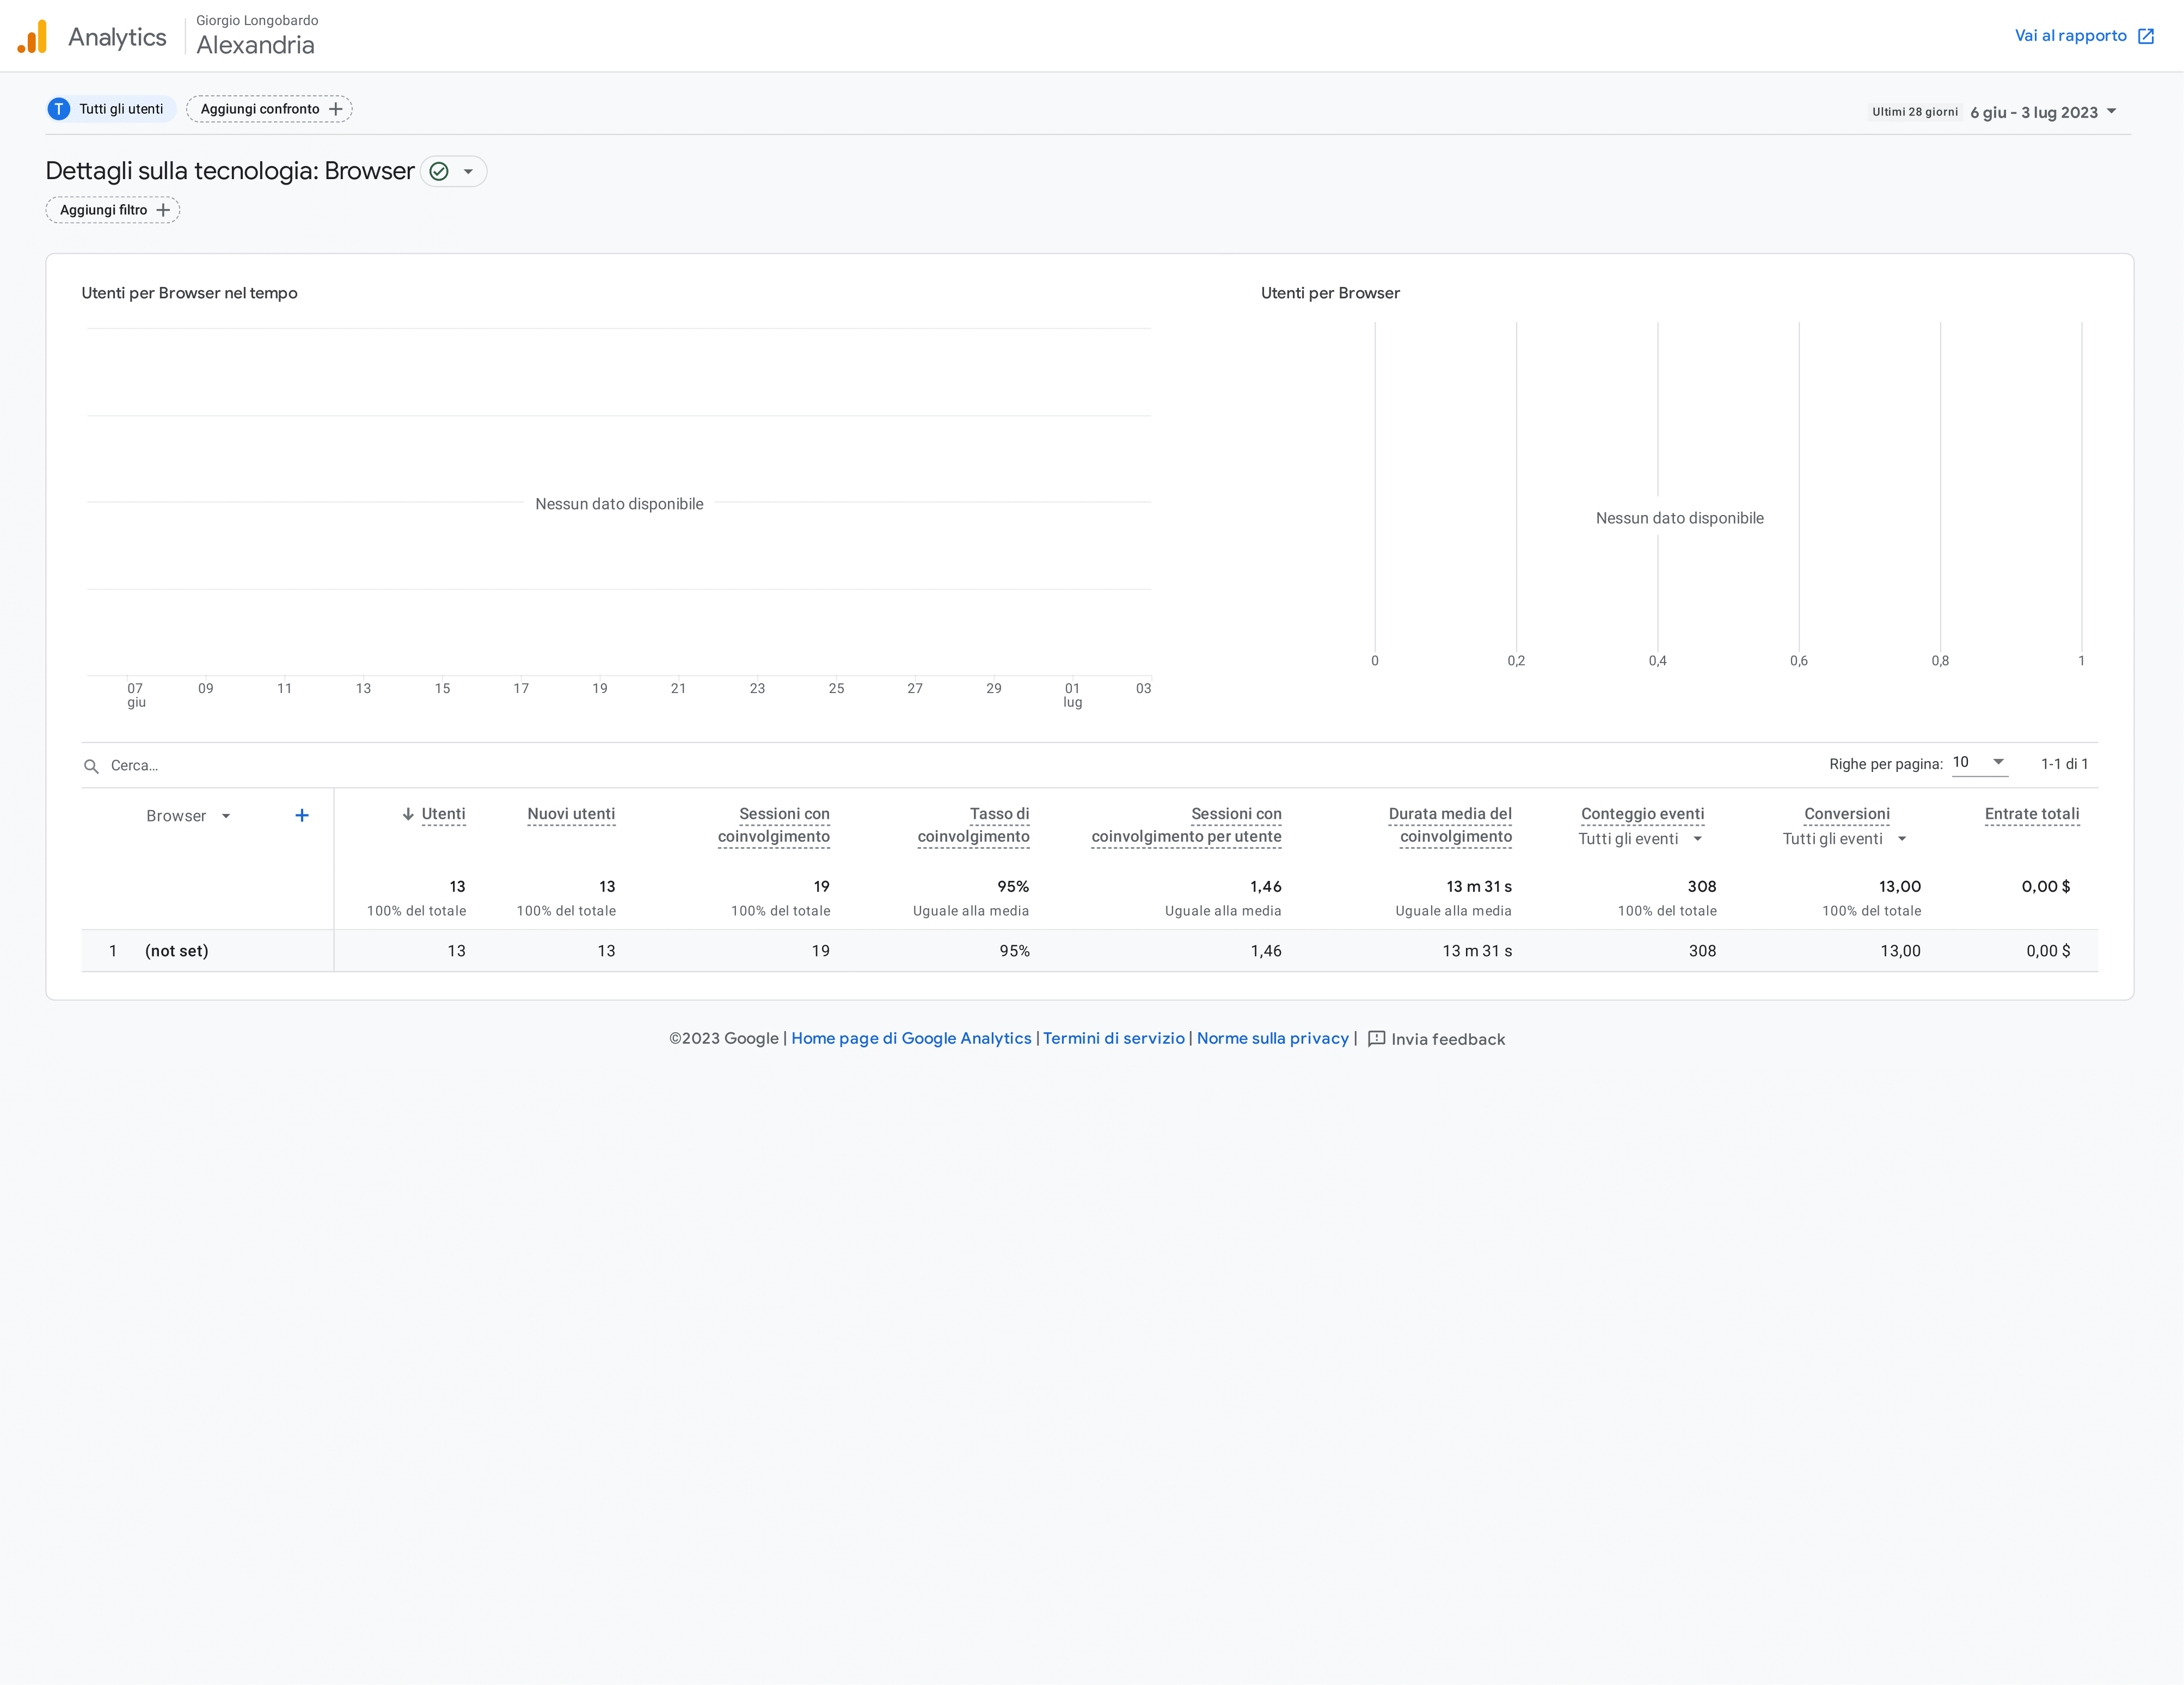
\includegraphics[width=0.99\textwidth]{Immagini/Alexandria/Report/dettagliTecnologia-1.png}
    \caption{Panoramica dettagli delle tecnologie}
\end{figure}

In particolare, abbiamo deciso principalmente di apportare due modifiche all'applicativo finale: la gradazione del colore principale dell'applicazione e migliorie alle schermate di controllo per aumentare \textit{l'affordance.} Abbiamo deciso di tenere traccia dei tasso di successo di pochi utenti per poi modificare eventualmente l'applicativo rendendolo più semplice. Ergo è stata compilata questa tabella:

\begin{table}[h]
\resizebox{\columnwidth}{!}{\begin{tabular}{|l|c|c|c|c|c|c|}
\hline
                      & \multicolumn{1}{l|}{Task 1: Ricerca Riferimento} & \multicolumn{1}{l|}{Task 2: Creazione Riferimento} & \multicolumn{1}{l|}{Task 3: Creazione Categoria} & \multicolumn{1}{l|}{Task 4: Modifica Riferimento} & \multicolumn{1}{l|}{Task 5: Visualizzazione di un Riferimento} & \multicolumn{1}{l|}{Task 6: Eliminazione Riferimento} \\ \hline
Utente 1              & S                                                & S                                                  & S                                                & P                                                 & S                                                              & S                                                     \\ \hline
Utente 2              & S                                                & S                                                  & P                                                & F                                                 & S                                                              & S                                                     \\ \hline
Utente 3              & S                                                & S                                                  & S                                                & S                                                 & S                                                              & S                                                     \\ \hline
Utente 4              & S                                                & S                                                  & S                                                & P                                                 & S                                                              & S                                                     \\ \hline
Utente 5              & S                                                & S                                                  & S                                                & P                                                 & S                                                              & P                                                     \\ \hline
Percentuale successo: & 100\%                                            & 100\%                                              & 90\%                                             & 45\%                                              & 100\%                                                          & 90\%                                                  \\ \hline
\end{tabular}}
\caption{Tasso di successo}
\end{table}
Dove S, F e P indicano rispettivamente Successo, Fallimento e Parziale (Successo). E' da precisare inoltre che la tabella non tiene conto del tempo impiegato per ogni utente a svolgere un determinato compito. Tutti gli utenti rivestono il ruolo di un normale utente, non godendo di particolari privilegi del sistema, ma solamente eventuale potere di creare categorie, riferimenti ed eliminare i propri oggetti realizzati.

Una volta analizzati i dati, abbiamo deciso di migliorare le schermate dei Task che generassero un basso tasso di successo. In questo caso, il compito \textit{Modifica Riferimento} genera un tasso di successo < 60\%, dove 60 è un tasso che consideriamo sufficiente per non modificare le schermate correlate. Dunque, la schermata per la modifica di un riferimento ha subito migliorie per evitare fraintendimenti o casi di insuccesso. 

    \chapter{Conclusione}
\raggedright{\section{Note finali}}
L'intero applicativo è stato realizzato da Giorgio Longobardo, Claudio Simonelli e Giuseppe Francione e tale documento rappresenta uno degli output richiesti dal committente, SoftEngUniNA, realizzata da Giorgio Longobardo, Claudio Simonelli e Giuseppe Francione. Vengono presentati tutti i dettagli progettuali di \textit{Alexandria}, applicazione deputata nella gestione di Riferimenti bibliografici. Il nome fa riferimento alla biblioteca di Alessandria, una antica città egiziana che ospitava una delle bibliotece più antiche al mondo. L'applicativo è stato sviluppato per soli fini didattici per il corso di Informatica della Federico II di Napoli. Tale documentazione contiene link al codice sorgente, al dockerfile e mockup di Figma.
\hspace{0pt}
\vfill
    \raggedleft Giorgio Longobardo \\ Giuseppe Francione \\ Claudio Simonelli
\vfill
\hspace{0pt}

    

\end{document}

    \centering\scshape\Medium\ UNIVERSITÀ DEGLI STUDI DI NAPOLI FEDERICO II\\
    \centering\scshape\small\ SCUOLA POLITECNICA E DELLE SCIENZE DI BASE\\
    \centering\scshape\Medium\ DIPARTIMENTO DI INGEGNERIA ELETTRICA E TECNOLOGIE DELL'INFORMAZIONE\\
            \begin{center}
        
            
\includegraphics[width=.25\textwidth]{Immagini/FedericoII.png}
        \end{center}


    \end{figure}
    


    \chapter{Introduzione}
\raggedright{\section{Descrizione richiesta del progetto}}

È richiesto di migliorare e potenziare un sistema informativo già esistente per la gestione di bibliografie. Il sistema deve essere capace di salvare e organizzare i riferimenti bibliografici degli utenti.  In particolare, è possibile inserire, modificare, rimuovere riferimenti bibliografici di diverso tipo (e.g.: articoli scientifici su conferenza o rivista, libri, risorse on-line, dataset, etc.).
Ciascun riferimento è caratterizzato da un titolo univoco, un elenco di autori, una data, un URL (obbligatorio solo per risorse on-line), un DOI (facoltativo, ma univoco ove presente), e una descrizione testuale in cui l’utente può indicare aspetti significativi.
Inoltre, un riferimento può essere associato a un insieme di rimandi, ovvero di altri riferimenti presenti nel sistema che vengono menzionati nel testo.

Un utente, infine, può definire un insieme di categorie personalizzate e possibilmente gerarchiche, e associare ciascun riferimento a una o più categorie. Per organizzazione gerarchica delle categorie si intende la possibilità di specificare che una certa categoria (e.g.: “Informatica”) ha una o più sottocategorie (e.g.: “Basi di Dati” o “Testing”).

Non è possibile introdurre dipendenze cicliche, ovvero non è possibile che una categoria sia una sottocategoria (anche transitivamente) di sé stessa. L’appartenenza a una sottocategoria implica l’appartenenza a tutte le sue super-categorie. Non è pertanto possibile associare esplicitamente a un riferimento una categoria e una sua super-categoria.

Il sistema permette infine di effettuare interrogazioni avanzate, con possibilità di filtraggio per una o più categorie, per data, per parole chiave e per autore. Inoltre, è possibile ordinare i riferimenti per numero di citazioni ricevute, ovvero per il numero di volte in cui il riferimento è presente nei rimandi di altri riferimenti.

Inoltre è richiesto lo sviluppo di nuove funzionalità da integrare nel sistema informativo già esistente.

\raggedright{\section{Stato progetto originale}}
L'applicativo originale, seppur lasciato in ottimo stato, presenta alcuni punti deboli per quanto riguarda la progettazione software e usabilità. In particolare, verranno mostrati le varie funzionalità e i vari aspetti dell'applicativo che verranno modificati affinché possa rispettare gli standard odierni.
\raggedright{{\subsection{Basi di dati}}}
         \begin{center}
     \hspace{-1cm}
            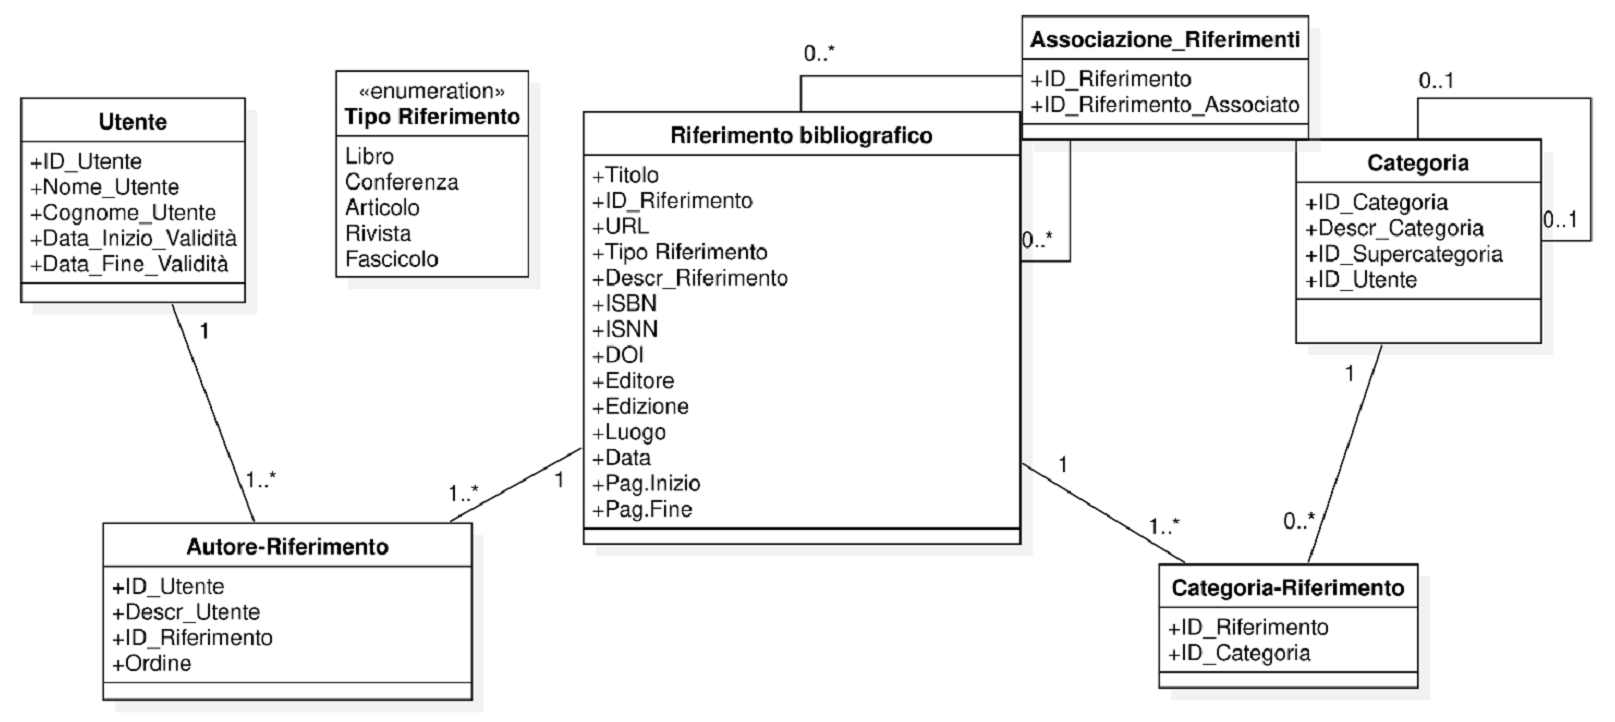
\includegraphics[width=.90\textwidth]{Immagini/VecchioProgetto/UML Basi di Dati pre ristrutturato.png} 
        \end{center}
La Basi di Dati originale è stata implementata nel modo seguente: \\la tabella \textit{Utente} descrive il possible utente che accede alla piattaforma dei riferimenti bibliografici. Contiene un identificativo univoco, un nome e cognome e due date di inzio e fine validità rispettivamente. \\
La tabella \textit{Autore-Riferimento} descrive il possible ideatore o relatore in base a che tipologia di riferimento bibliografico si analizzi. \\
La tabella \textit{Riferimento Bibliografico} descrive il possible riferimento bibliografico e le sue caratteristiche in base alla tipologia. \\
La tabella \textit{Categoria} descrive una categoria e le sue possibili sottocategorie. \\
La tabella \textit{Associazione-Riferimenti} è un descrittore di un riferimento che può essere associato a un insieme di rimandi. \\
La tabella \textit{Categoria-Riferimento} è un descrittore di una categoria che è associata ad  un riferimento. \\
\raggedright{\subsection{Applicativo Java}}
L’approccio di design utilizzato è quello di un sistema Object Oriented sviluppato in Java che dipende strettamente da un database PostgreSQL. L’ambiente di sistema è un qualsiasi sistema operativo non-mobile (quindi desktop) fornito di una connessione al database.
\begin{center}
    \hspace{-1cm}
        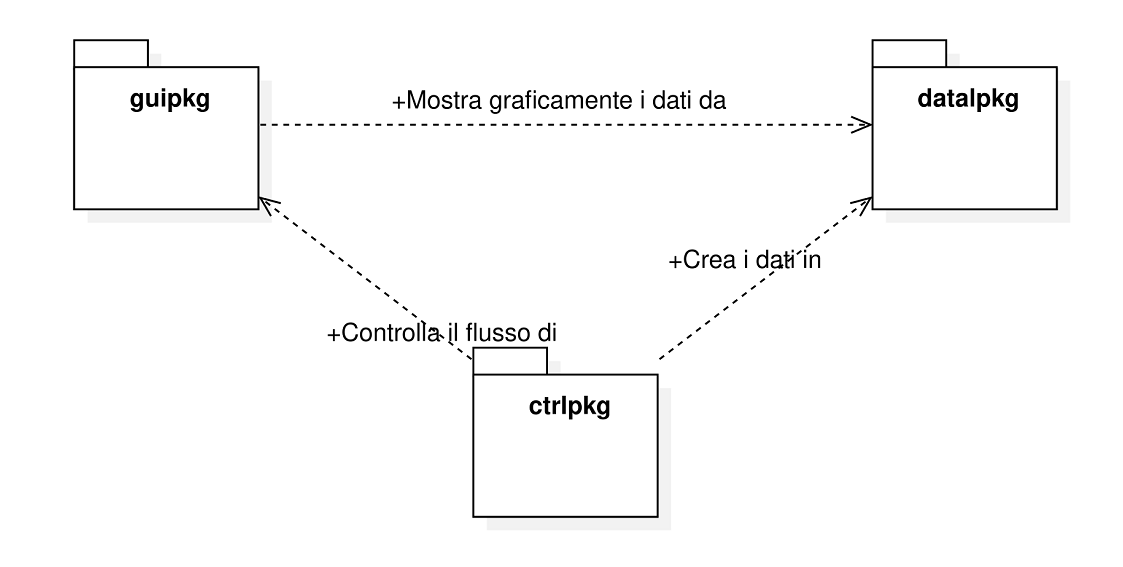
\includegraphics[width=.90\textwidth]{Immagini/VecchioProgetto/UML OO Java vecchioProgetto.png} 
\end{center}

Il sistema è costituito da 3 elementi principali, rappresentati in package: \\
\textit{guipkg}, per la definizione delle interfacce grafiche e le loro interazioni; \\ 
\textit{datalpkg}, per la definizione delle classi di dati che andranno trattati e mostrati;\\
\textit{ctrlpkg}, per la definizione dei collegamenti e delle varie interazioni tra sistema e database esterno.

\raggedright{\section{Migliorie del progetto originale e nuove funzionalità}}
La nuova versione del progetto prevede la modifica delle seguenti funzionalità:
\begin{itemize}
    \item Nuovo sistema di accesso: il sistema non prevederà l'utilizzo dell'ID utente ma di una email e password apposita. Durante la registrazione verrà richiesto infatti di inserire le due informaizoni che saranno poi salvate nel database. Inoltre, per preservare la sicurezza degli utenti, le password verranno criptate.
    \item Rimozione visibilità di ID accesso durante la registrazione: poiché l'utente non può più sapere il suo identificativo, non verrà mostrato il suo ID durante la registrazione.
    \item Potenziamento modalità di ricerca: la ricerca di riferimenti, citazioni e categorie verrà modificato e sarà più intuitivo ed efficiente.
    \item Apertura collegamenti: l'applicativo sarà capace di aprire gli URL inseriti per migliorare l'esperienza dell'utente, funzionalità mancante dell'applicativo originale.
    \item Impostazioni utente: verrà aggiunta la possibilità di modificare le proprie credenziali mediante un menù apposito.
    \item Miglioramento dell'interfaccia grafica: la GUI sarà totalmente ridisegnata per rispettare criteri di buona usabilità e con lo scopo di migliorare l'affordance iniziale, in tal modo da poter soddisfare più utenti possibili e di coprire tutte le possibili esigenze.
\end{itemize}


\end{document}